\documentclass[12pt,a4paper]{article}
%\usepackage[utf8]{inputenc}
%\usepackage[portuguese]{babel}
\usepackage{amsmath, amsfonts, amssymb}
\usepackage{graphicx}
\usepackage[utf8]{inputenc} % Permite utilizar caracteres especiais: Ex: ç á à...
\usepackage[onehalfspacing]{setspace} % Espaçamento de 1,5
\usepackage{cabecalho}
\usepackage{multirow}
\usepackage[lmargin=3cm, tmargin=3cm, rmargin=2cm, bmargin=2cm]{geometry}
\usepackage{indentfirst}
\usepackage[brazilian]{babel} % Traduzir para PT-BR
\usepackage{IEEEtrantools}
% Alguns comas
\newcommand{\rxy}{{\mathit{\mathbf{R}}}_{\mathit{x\mathbf{y}}}}
\newcommand{\ry}{{\mathit{\mathbf{R}}}_{\mathit{\mathbf{y}}}}
\newcommand{\wo}{\mathit{\mathbf{w_o}}}
\newcommand{\wn}{\mathit{\mathbf{w}}\left\lbrack n\right\rbrack}
\newcommand{\vn}{\mathit{\mathbf{v}}\left\lbrack n\right\rbrack}

\begin{document}
	\initcab{Universidade Federal do Ceará}{Estimação e Detecção}{Chales Casimiro Cavalcante}{474725}{Dezembro de 2019}{Lista 6}

\begin{enumerate}
\item
\begin{enumerate}
\item
O vetor variáveis aleatórias $\mathbf{y}$ é definido por
	\begin{IEEEeqnarray}{rCl}
	\mathit{\mathbf{y}} & = & \left\lbrack \begin{array}{c}
y\left\lbrack n\right\rbrack \\
y\left\lbrack n-1\right\rbrack 
\end{array}\right\rbrack		
	\end{IEEEeqnarray}

	Em que $y\left\lbrack n\right\rbrack$ é a saída de um canal do comunicação (definida pela função de sistema $H(z)$) para um sinal de entrada $x[n]$. Seja a função de sistema do canal dada por:
	\begin{IEEEeqnarray}{rCl}
	H\left(z\right)& = & 1+1,6z^{-1}
	\label{hz}
	\end{IEEEeqnarray}
	
	A transformada Z da saída do sistema é:
	\begin{IEEEeqnarray}{rCl}
	Y\left(z\right) & = & X\left(z\right)H\left(z\right) \nonumber \\
	& = & X\left(z\right)+1\ldotp 6z^{-1} X\left(z\right)
	\label{yz}
	\end{IEEEeqnarray}
	
	Aplicando a transformada Z inversa em \ref{yz}, temos:
	\begin{IEEEeqnarray}{rCl}
	y\left\lbrack n\right\rbrack =x\left\lbrack n\right\rbrack +1,6x\left\lbrack n-1\right\rbrack
	\label{yn}
	\end{IEEEeqnarray}
	
	Com base na equação \ref{yn}, a matriz de correlação é:
	\begin{IEEEeqnarray}{rCl}
	\ry & = & \left\lbrack \begin{array}{cc}
E\left\lbrace y^2 \left\lbrack n\right\rbrack \right\rbrace  & E\left\lbrace y\left\lbrack n\right\rbrack y\left\lbrack n-1\right\rbrack \right\rbrace \\
E\left\lbrace y\left\lbrack n-1\right\rbrack y\left\lbrack n\right\rbrack \right\rbrace  & E\left\lbrace y^2 \left\lbrack n-1\right\rbrack \right\rbrace 
\end{array}\right\rbrack \nonumber \\
	& = &\left\lbrack \begin{array}{cc}
	3,56 & 1,6\\
	1,6 & 3,56
\end{array}\right\rbrack
	\label{ry}
	\end{IEEEeqnarray}
	
	E a matriz de correlação cruzada entre o sinal desejado e o sinal de entrada é:
	\begin{IEEEeqnarray}{rCl}
	\rxy & = & E\left\lbrace \mathit{\mathbf{y}}\;x\left\lbrack n\right\rbrack \right\rbrace \nonumber \\
	& = & \left\lbrack \begin{array}{c}
E\left\lbrace y\left\lbrack n\right\rbrack x\left\lbrack n\right\rbrack \right\rbrace \\
E\left\lbrace y\left\lbrack n-1\right\rbrack x\left\lbrack n\right\rbrack \right\rbrace 
\end{array}\right\rbrack \nonumber \\
	& = & \left\lbrack \begin{array}{c}
1\\
0
\end{array}\right\rbrack
	\label{rxy}
	\end{IEEEeqnarray}	

	As equações de Wiener busca os coeficientes do filtro FIR (do inglês, \textit{Finite Impulse Response}) que minimiza a função custo:
	\begin{IEEEeqnarray}{rCl}
	J\left(\mathit{\mathbf{w}}\right)& = & E\left\lbrack e^2 \left\lbrack n\right\rbrack \right\rbrack
	\end{IEEEeqnarray}
	
	Em que $\mathbf{w}$ são os seus coeficientes e $e[n]$ é o sinal de erro entre a saída do filtro e o sinal desejado. No contexto dessa questão, deseja-se obter o filtro de de Wiener que desempenhe a função de equalização de canal, isto é, busca-se obter os coeficiente da filtragem ótima que seja capaz de recuperar o máximo possível o sinal transmitido, $x[n]$. Aplicando a equação de Wiener-Hopf, temos:
	\begin{IEEEeqnarray}{rCl}
	\wo &= &{{\mathit{\mathbf{R}}}_{\mathit{\mathbf{y}}} }^{-1} {\mathit{\mathbf{R}}}_{\mathit{\mathbf{xy}}} \nonumber \\
	&= & \left\lbrack \begin{array}{c} 0,352\\ -0,1582 \end{array}\right\rbrack
	\label{woIta}
	\end{IEEEeqnarray}
	
	Para provar a eficácia da filtragem ótima aplicado à equalização de canal, é gerado (em ambiente computacional) um sinal branco, de variância unitária para representar o sinal transmitido $x[n]$. Este processo aleatório passa por um canal cuja função de sistema é igual a equação \ref{hz}. Com o objetivo de recuperar o sinal transmitido, é utilizado um filtro de Wiener no receptor com os parâmetros iguais aos que foram calculados na equação \ref{woIta}. A Figura \ref{ita} mostra o resultado desse processamento.
	
	\begin{figure}[hbt]
	\centering
	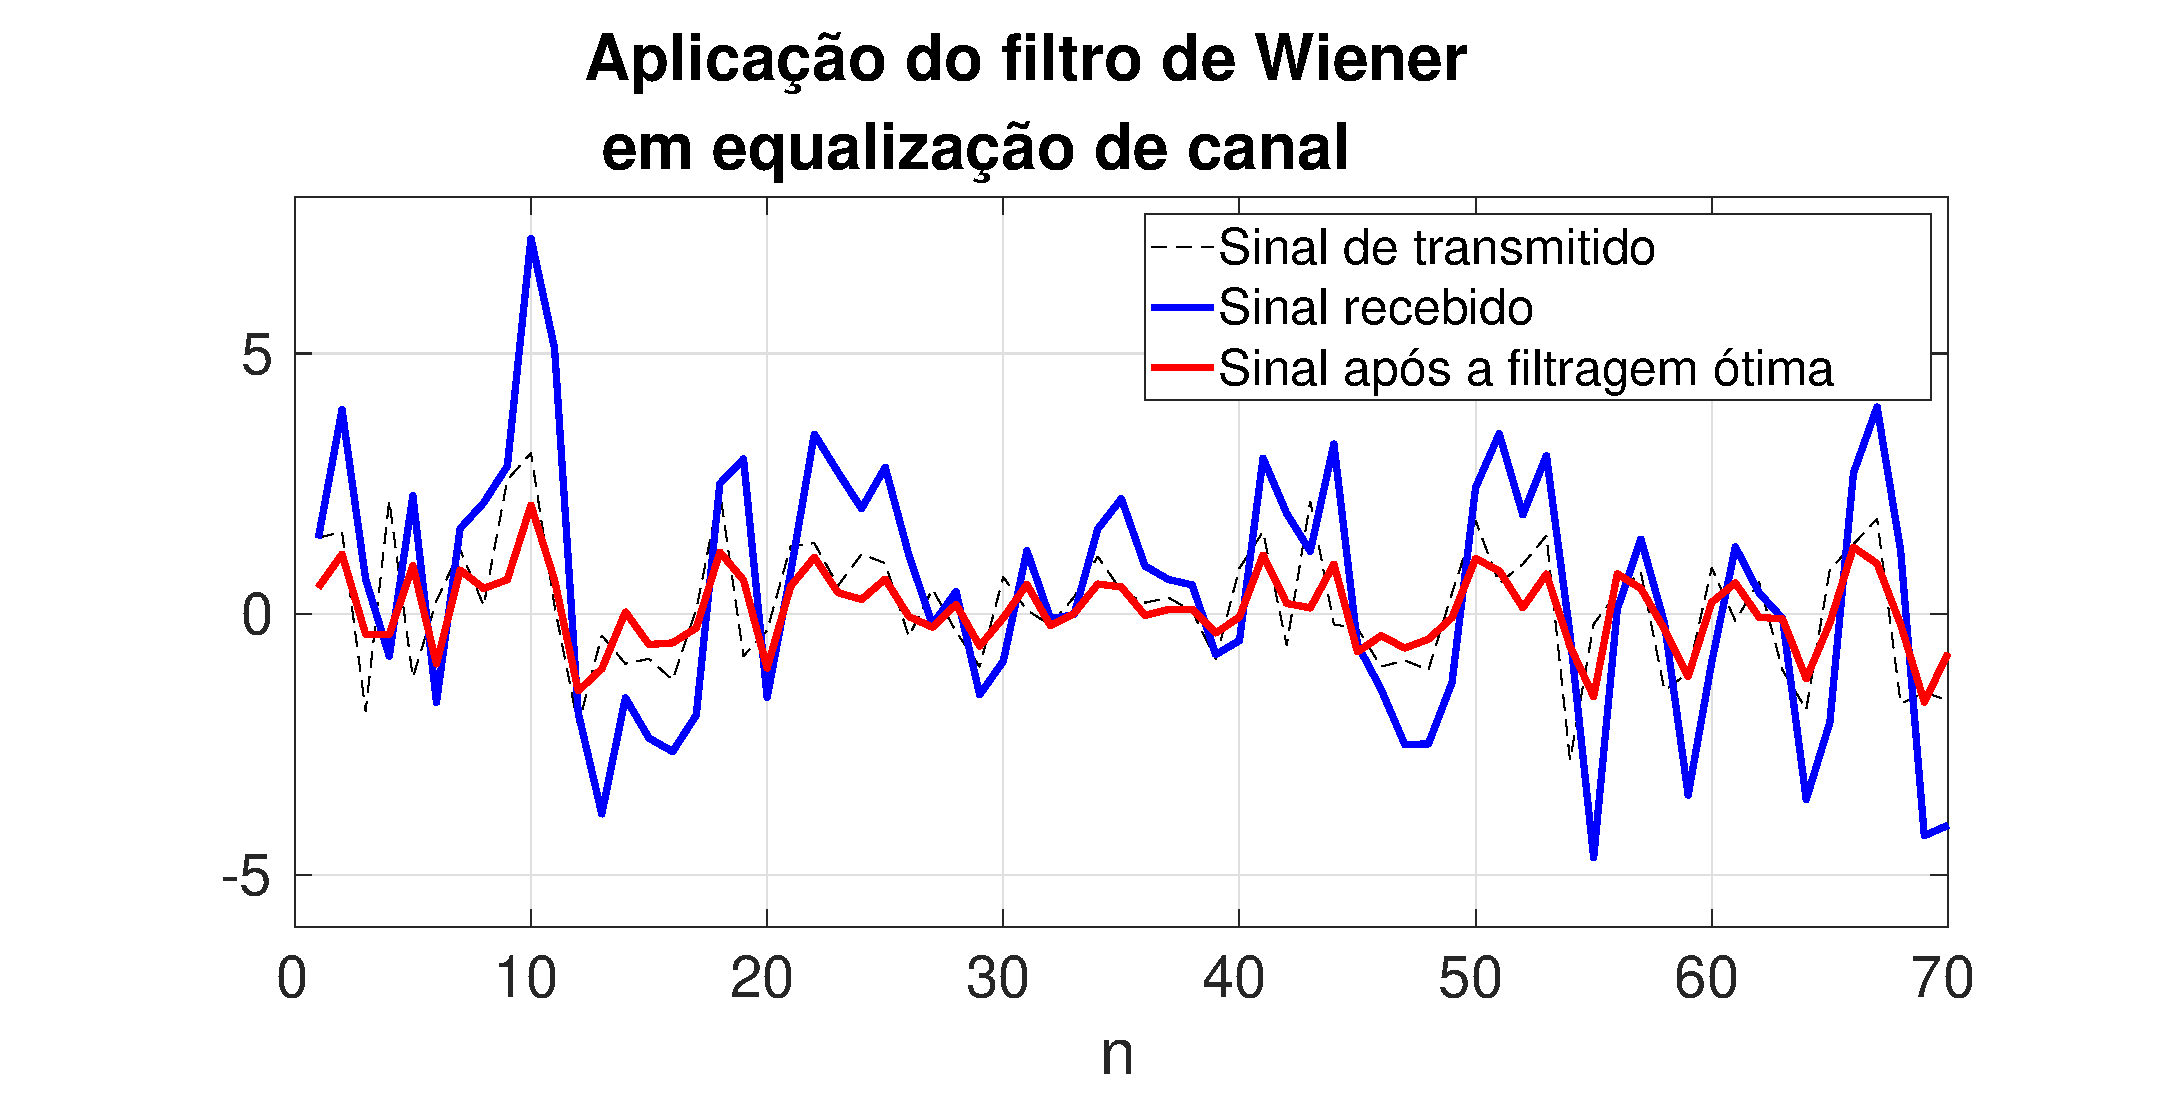
\includegraphics[scale=.4]{figs/wiener.eps}
	\caption{Processamento do sinal recebido utilizando o filtro de Wiener (equalização de canal).}
	\label{ita}
	\end{figure}
	
	Como é possível perceber, o filtro de Wiener aproxima significativamente $y[n]$ a $x[n]$. Canais com memória são comumente encontrados em sistemas de comunicações reais. A filtragem ótima provê uma ótima ferramenta prática para a equalização canais com mais de 1 \textit{tap} de duração.
	
	\item
	\begin{enumerate}
	\item
		Para o cálculo do algoritmo do gradiente, pretende-se calcular o seguinte:
		\begin{enumerate}
			\item Decomposição de $\ry$
			\item Modos naturais
			\item Equações do aprendizado do filtro
		\end{enumerate}
		
		A matriz modal (i.e., a matriz formada pelos autovetores ortogonais) é dada por \cite{MouradBarkat}:
		\begin{IEEEeqnarray}{rCl}
			\mathbf{Q} & = &\left\lbrack \begin{array}{cc}
-0,7071 & 0,7071\\
0,7071 & 0,7071
\end{array}\right\rbrack
			\label{Q}
		\end{IEEEeqnarray}
		
		A matriz diagonal dos autovalores é:
		\begin{IEEEeqnarray}{rCl}
			\mathbf{\Lambda} & = & \left\lbrack \begin{array}{cc}
1,96 & 0\\
0 & 5,16
\end{array}\right\rbrack
		\end{IEEEeqnarray}
		
		Os coeficientes do filtro adaptativo aproximam-se dos coeficientes ótimos, $\wo$, de acordo com os modos naturais. Para que o algoritmo convirja, é necessário que os modos naturais tendam a 0 a medida que o laço do algoritmo é incrementado. O vetor dos modos naturais é dado por \cite{SilvioAbrantes}:
	\begin{IEEEeqnarray}{rCl}
	\vn =\left\lbrack \begin{array}{c}
v_0 \left\lbrack n\right\rbrack \\
v_1 \left\lbrack n\right\rbrack 
\end{array}\right\rbrack ={\mathit{\mathbf{Q}}}^T {\mathit{\mathbf{w}}}_{\mathit{\mathbf{e}}}
	\end{IEEEeqnarray}
	
	Em que ${\mathit{\mathbf{w}}}_{\mathit{\mathbf{e}}}=\wn - \wo$. Como $\mathit{\mathbf{w}}\left\lbrack 0\right\rbrack=\mathbf{0}$ (em que $\mathbf{0}$ é o vetor nulo), temos que:
	\begin{IEEEeqnarray}{rCl}
	\mathit{\mathbf{v}}\left\lbrack 0\right\rbrack &=&-{\mathit{\mathbf{Q}}}^T {\mathit{\mathbf{w}}}_o \nonumber \\
	&=& \left\lbrack \begin{array}{c}
0,36\\
-0,137
\end{array}\right\rbrack
	\end{IEEEeqnarray}
		
	Com base nos valores iniciais dos modos naturais, podemos calcular $\vn$ como segue:
	\begin{IEEEeqnarray}{rCl}
	\vn &=& {\left(\mathit{\mathbf{I}}-2\mu \Lambda \right)}^n \mathit{\mathbf{v}}\left\lbrack 0\right\rbrack\nonumber \\
	&=& \left\lbrack \begin{array}{c}
1,96\times 0,{804}^n \\
0
\end{array}\right\rbrack
	\end{IEEEeqnarray}
	
	Em que $\mu=0,05$ é o passo de adaptação. Por fim, o algoritmo recursivo do filtro é:
	\begin{IEEEeqnarray}{rCl}
	\mathit{\mathbf{w}}\left\lbrack n\right\rbrack & = &{\mathit{\mathbf{w}}}_{\mathit{\mathbf{o}}} +\sum_{j=0}^1 {\mathit{\mathbf{q}}}_{\mathit{\mathbf{j}}} v_j \left\lbrack n\right\rbrack {\left(1-2\mu \lambda_j \right)}^n \nonumber \\
	& = & \left\lbrack \begin{array}{c}
0,352-0,2551\times 0,{804}^n -0,0969\times 0,{484}^n \\
-0,1582+0,2551\times 0,{804}^n -0,0969\times 0,{484}^n 
\end{array}\right\rbrack
	\end{IEEEeqnarray}
	
	A Figura \ref{gradiente} mostra a curva de nível para o algoritmo gradiente. Como referência, também é colocado o poto de Wiener.
	\begin{figure}[hbt]
		\centering
		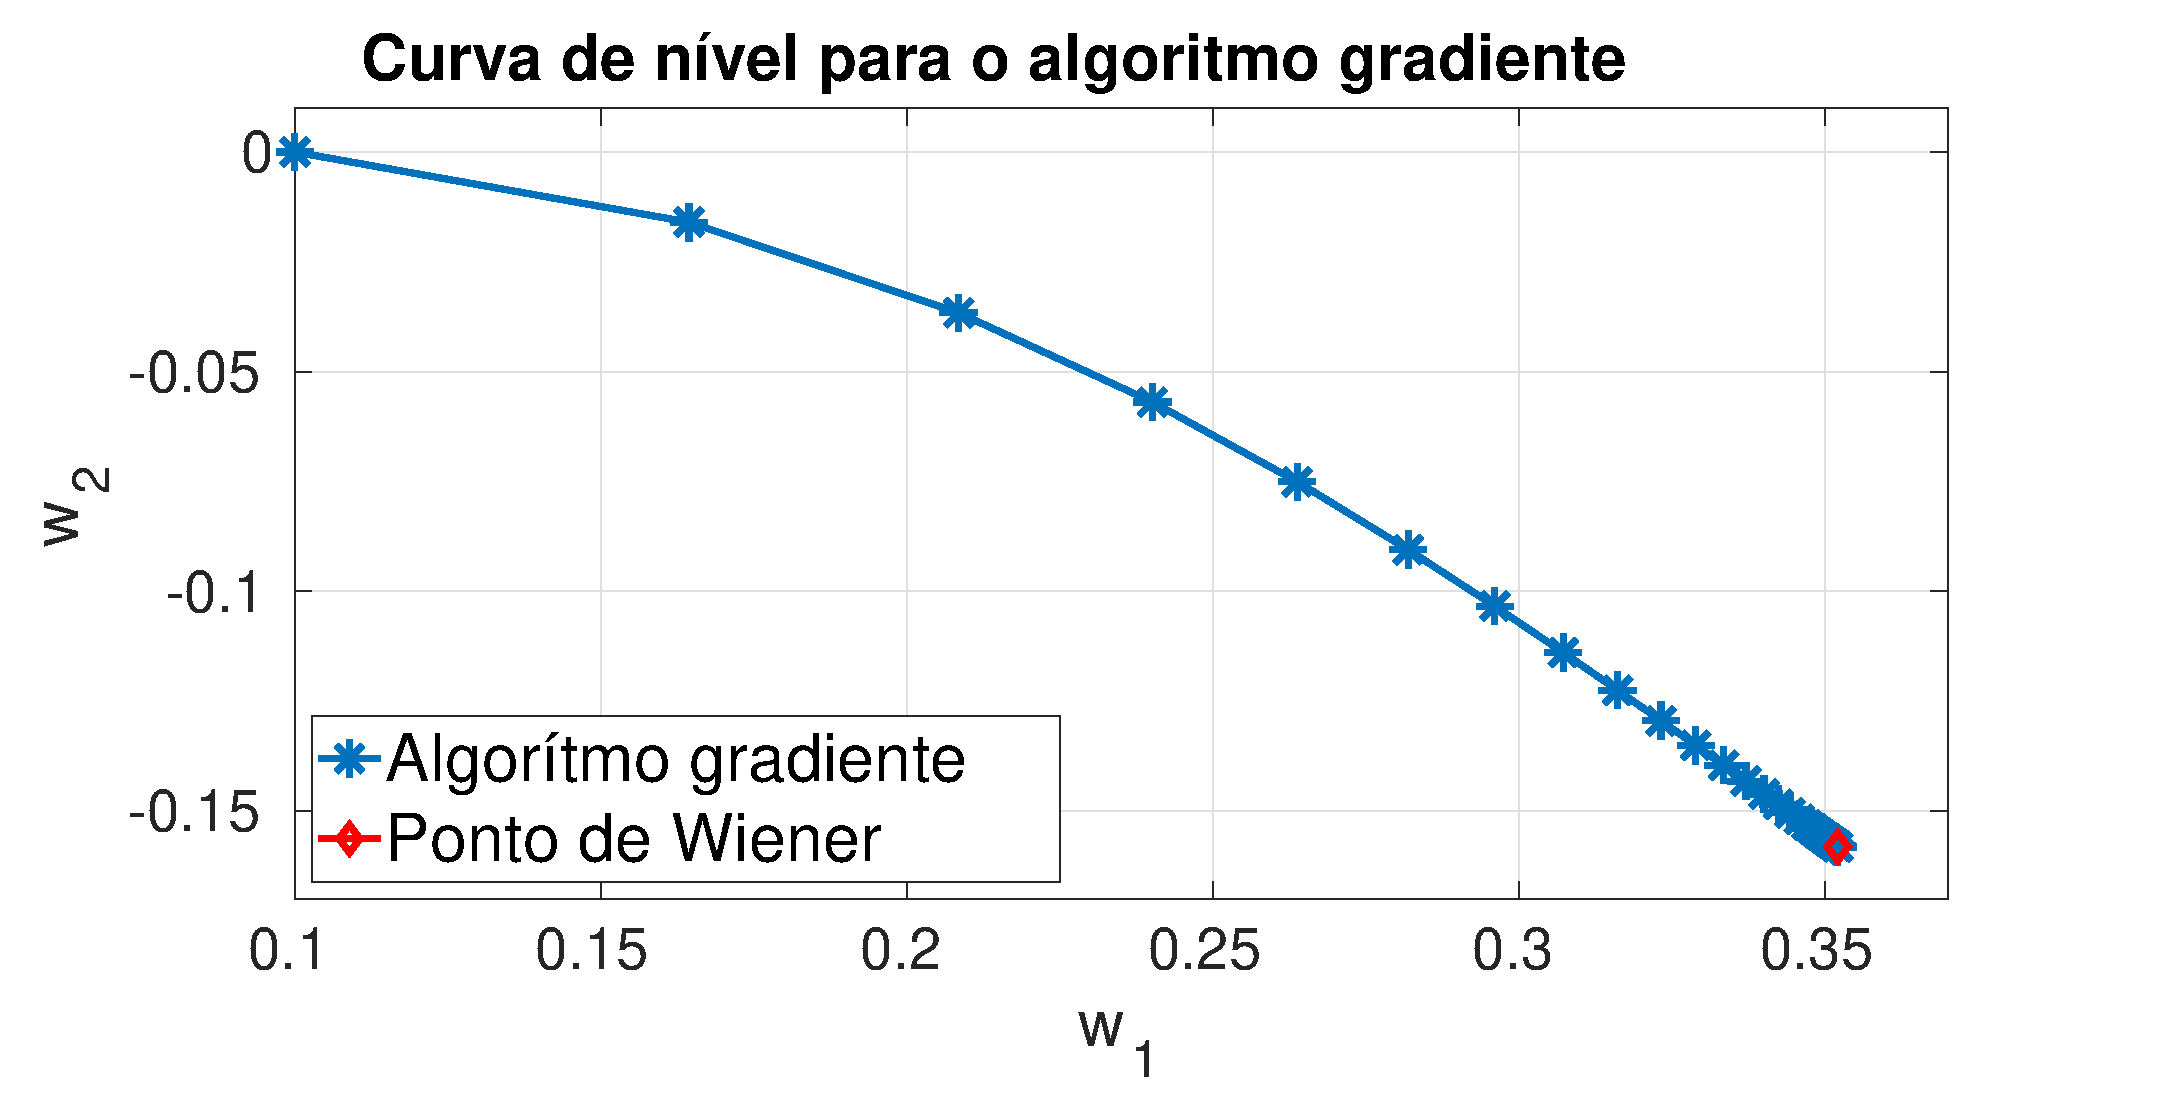
\includegraphics[scale=0.42]{figs/gradiente.eps}
		\caption{Curva de nível para o algoritmo gradiente.}
		\label{gradiente}
	\end{figure}
	\item
	Para o algoritmo de Newton, temos que:
	\begin{IEEEeqnarray}{rCl}
		\mathit{\mathbf{w}}\left\lbrack n+1\right\rbrack =\mathit{\mathbf{w}}\left\lbrack n\right\rbrack -\mu \left\lbrack \mathit{\mathbf{w}}\left\lbrack n\right\rbrack -{{\mathit{\mathbf{R}}}_{\mathit{\mathbf{y}}} }^{-1} {\mathit{\mathbf{R}}}_{\textrm{xy}} \right\rbrack
	\end{IEEEeqnarray}
	
	A Figura \ref{newton} mostra a curva de nível para este algoritmo.
	\begin{figure}[hbt]
		\centering
		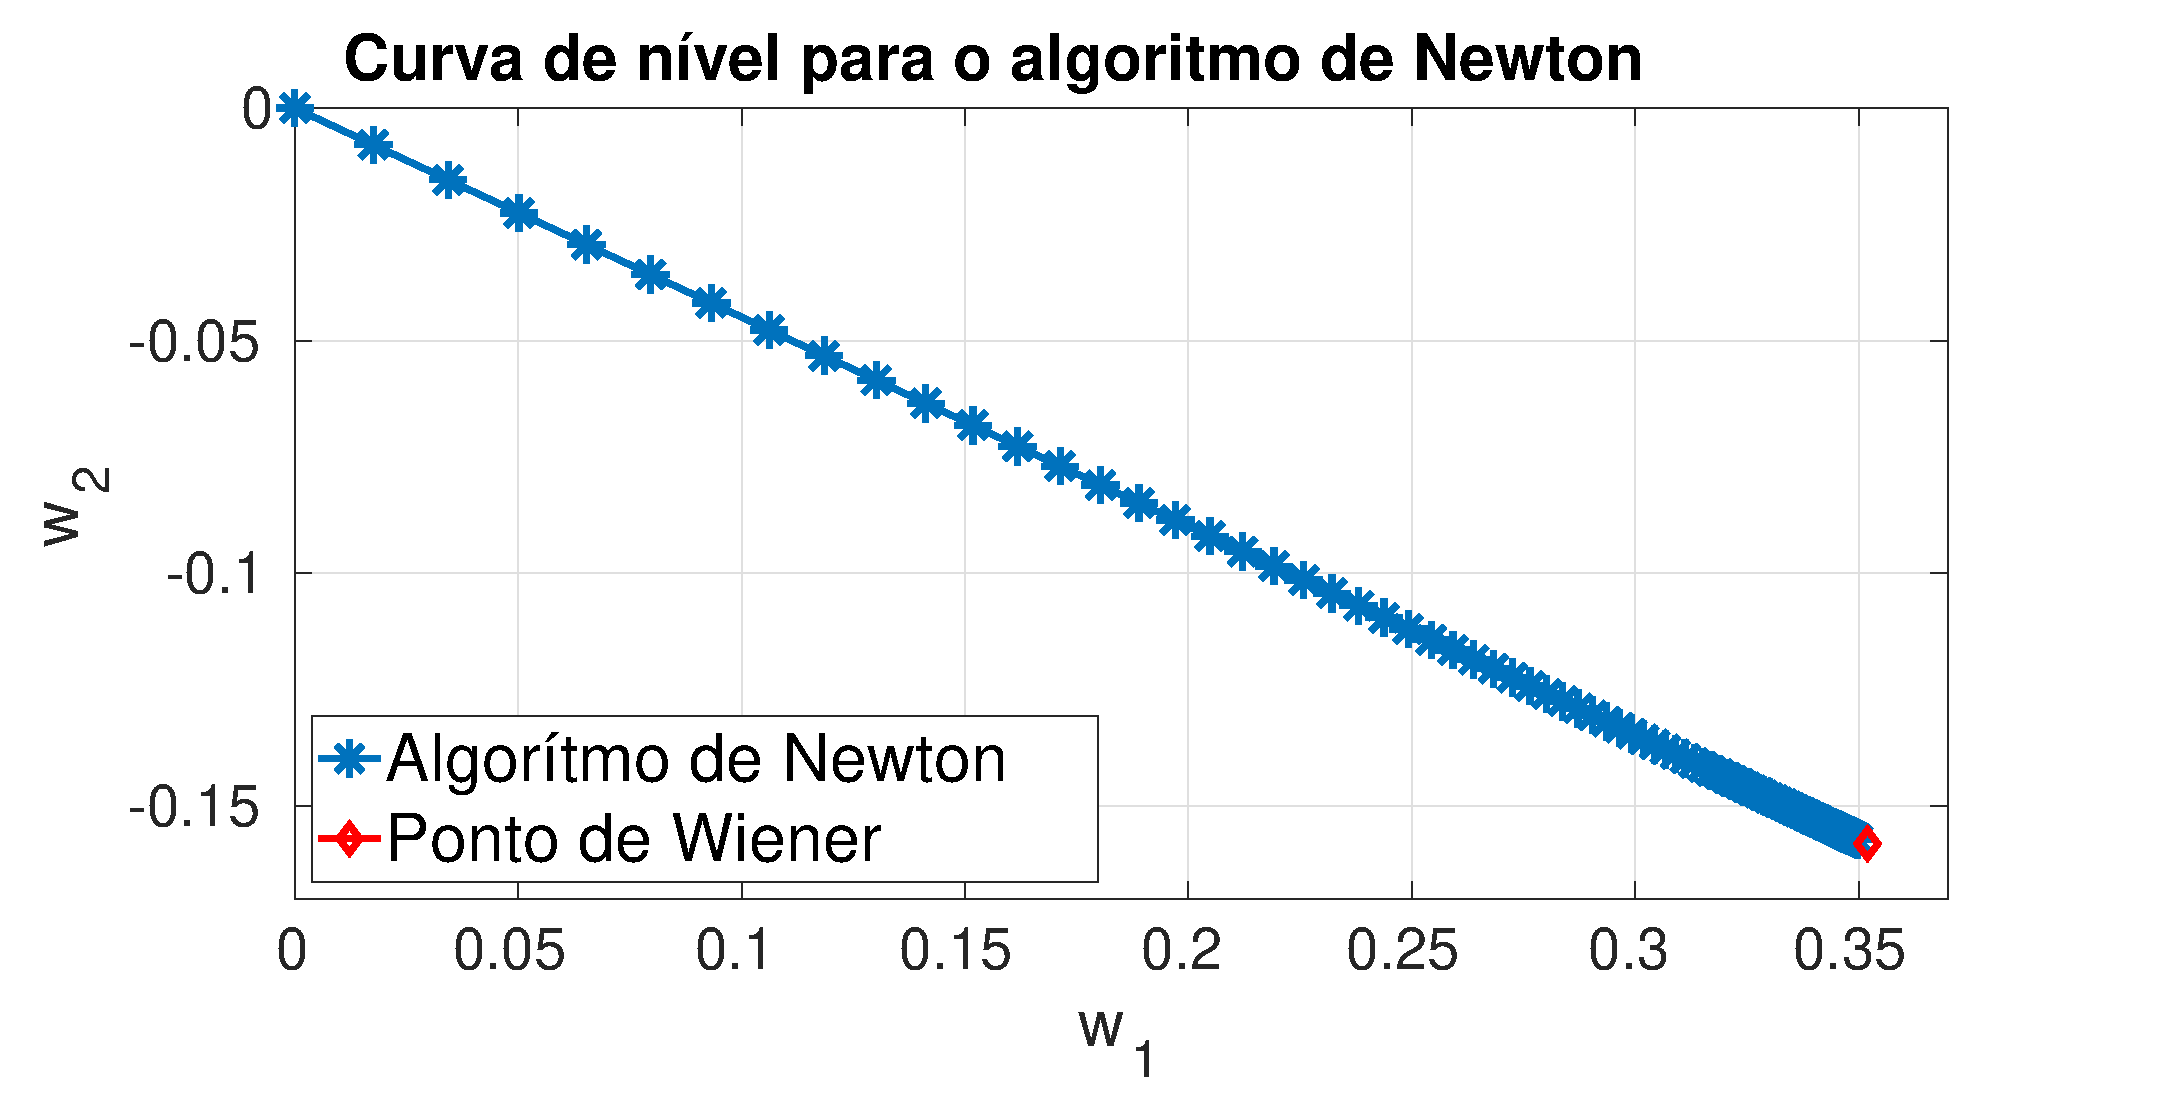
\includegraphics[scale=0.42]{figs/newton.eps}
		\caption{Curva de nível para o algoritmo de Newton.}
		\label{newton}
	\end{figure}
	
	Observe que, diferentemente da Figura \ref{gradiente}, a curva de superfície do algoritmo de Newton forma uma única reta até o ponte de Wiener. Isso se dá porque este algoritmo, por ser de segunda ordem, busca o caminho de minimiza a função custo em uma concavidade, enquanto que o gradiente busca em um plano. Como a função custo é quadrática, a curva de nível que vemos no algoritmo de Newton é um único segmento que nos leva até o ponto ótimo (após algumas iterações).
	
	\item
	
	Para o algoritmo LMS, o algoritmo de recursão é dado por:
	\begin{IEEEeqnarray}{rCl}
	\mathit{\mathbf{w}}\left\lbrack n+1\right\rbrack =w\left\lbrack n\right\rbrack +2\mu \mathit{\mathbf{x}}\left\lbrack n\right\rbrack e\left\lbrack n\right\rbrack
	\end{IEEEeqnarray}
	
	A Figura \ref{lms} mostra a curva de superfície para este algoritmo. Observe que, diferente dos outros algoritmos, o método LMS não obtém os coeficientes de Wiener perfeitamente. Ao invés, os coeficientes do filtro ótimo variam em torno do valor ótimo. Esse resultado está de acordo com o que é reportado na literatura.
	
	\begin{figure}[hbt]
	\centering
	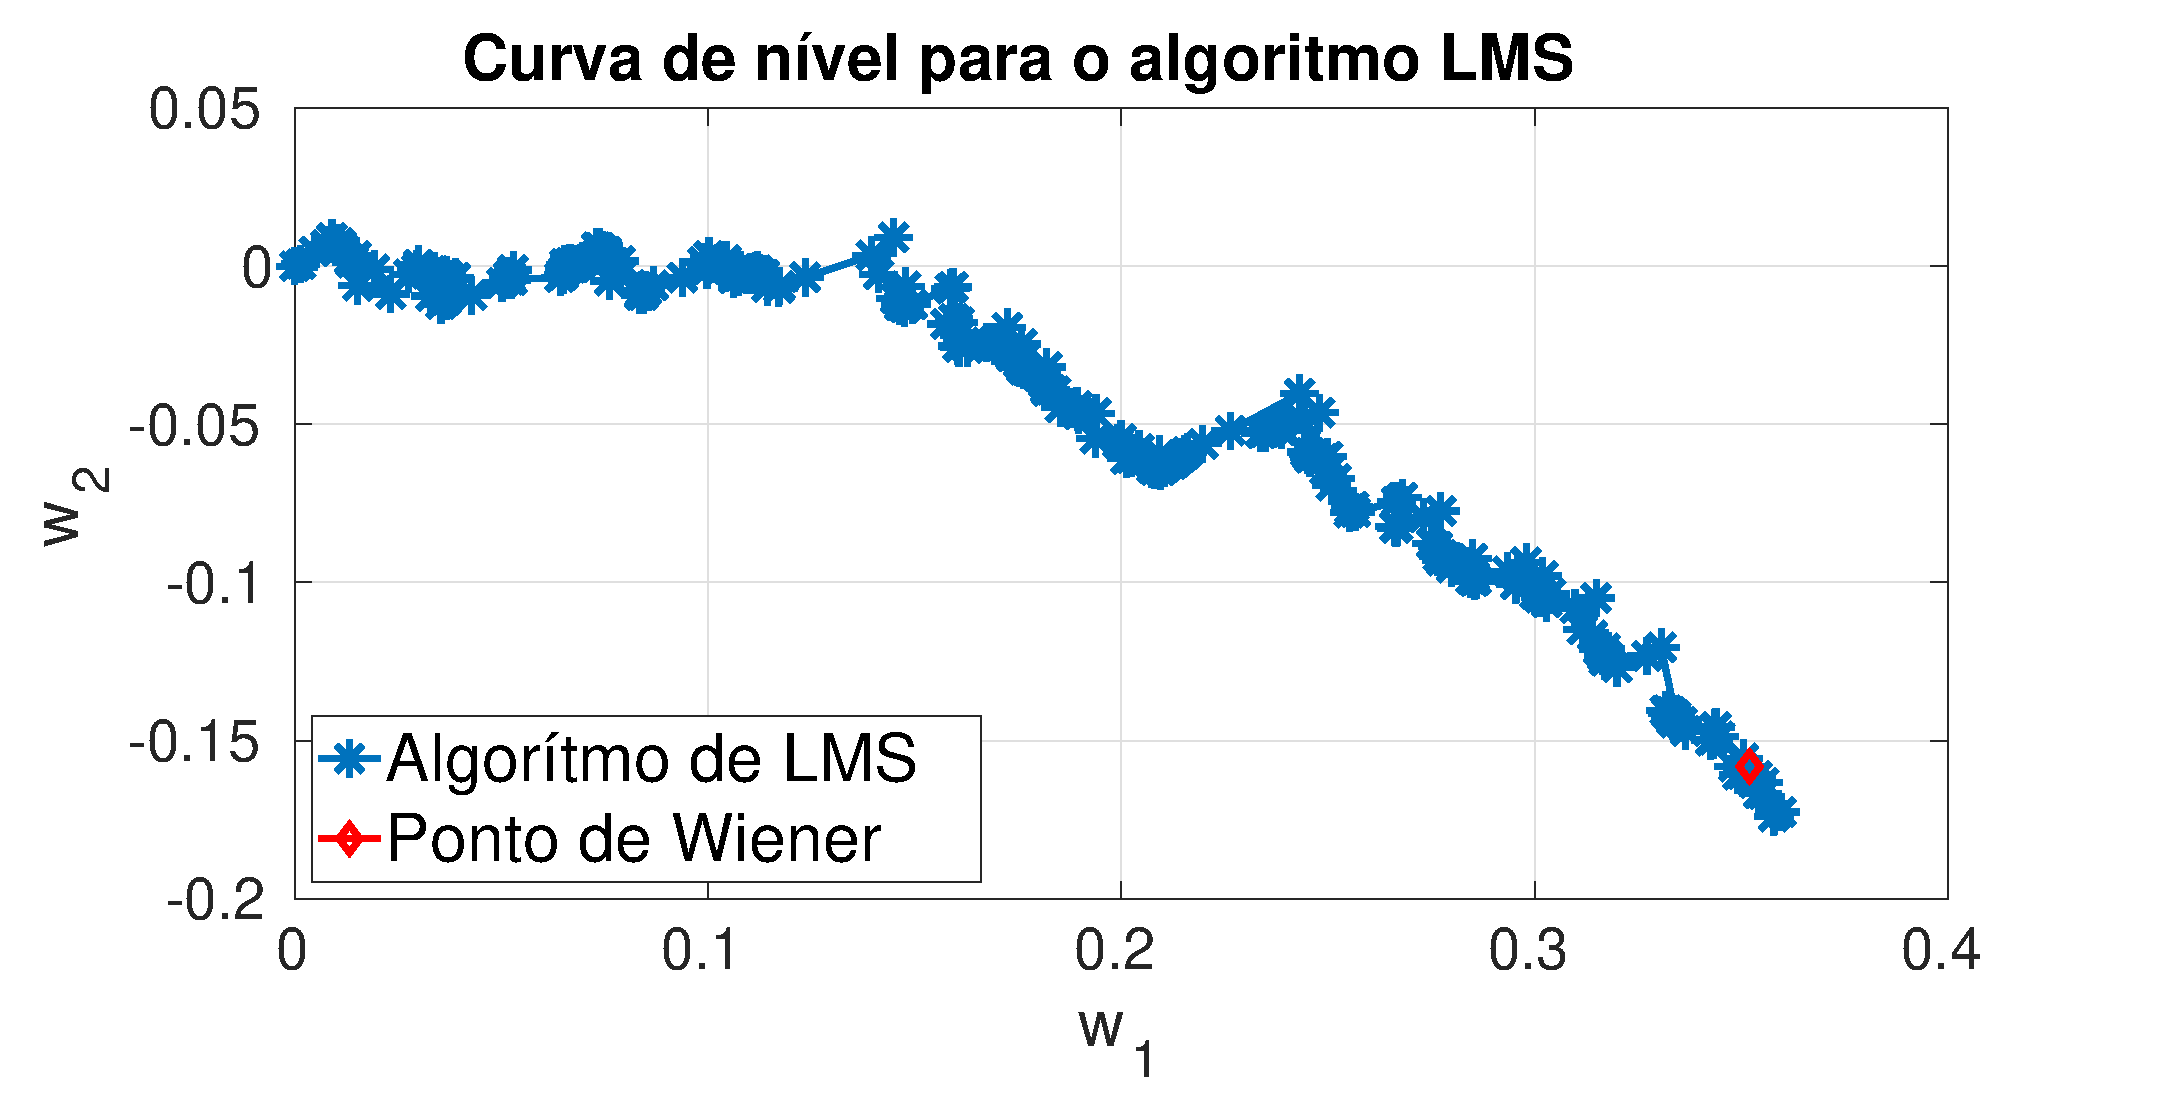
\includegraphics[scale=0.44]{figs/lms.eps}
	\caption{Curva de superfície para o algoritmo LMS.}
	\label{lms}
	\end{figure}
	
	\end{enumerate}
\end{enumerate}
\end{enumerate}

\bibliography{ref.bib}
\bibliographystyle{ieeetr}

\end{document}